\documentclass[11pt]{article}
\usepackage[margin=1in]{geometry}
\usepackage[utf8]{inputenc}
\usepackage[T1]{fontenc}
\usepackage{helvet}
\usepackage{booktabs, tabularx, multirow}
\usepackage{enumitem}
\usepackage{hyperref}
\usepackage{fancyhdr}
\usepackage{graphicx}
\usepackage{xcolor}
\usepackage{minted}
\usepackage{titling}
\usepackage[bottom]{footmisc}
\usepackage{titlesec}
\usepackage{parskip}
\usepackage{amsmath}
\usepackage{listings}
\usepackage{tcolorbox}
\usepackage{tikz}
\usetikzlibrary{shapes.geometric, arrows.meta, positioning}

\definecolor{primaryblue}{RGB}{0, 102, 204}
\definecolor{secondarygray}{RGB}{80, 80, 80}
\definecolor{codebg}{RGB}{245, 245, 245}
\definecolor{notebg}{RGB}{230, 240, 255}

\hypersetup{
    colorlinks=true,
    linkcolor=primaryblue,
    filecolor=magenta,
    urlcolor=cyan,
    pdftitle={1-Month Expert Architecture Training},
    bookmarks=true,
}

\pagestyle{fancy}
\fancyhf{}
\rhead{\textbf{Expert Architecture Training}}
\lhead{\textbf{ISYGO Consulting Services}}
\rfoot{\textit{Inspire Success, Your Goals \& Opportunities} | Page \thepage}

\titleformat{\section}{\Large\bfseries\sffamily\color{primaryblue}}{\thesection}{1em}{}
\titleformat{\subsection}{\large\bfseries\sffamily\color{secondarygray}}{\thesubsection}{1em}{}
\titleformat{\subsubsection}{\normalsize\bfseries\sffamily\color{secondarygray}}{\thesubsubsection}{1em}{}

\setlist[itemize]{noitemsep,topsep=4pt}
\setlist[enumerate]{noitemsep,topsep=4pt}

\lstset{
  backgroundcolor=\color{codebg},
  basicstyle=\small\ttfamily,
  frame=single,
  breaklines=true,
}

\newtcolorbox{technote}{colback=notebg, colframe=primaryblue, boxrule=0.5pt, arc=5pt, left=10pt, right=10pt, top=10pt, bottom=10pt}
\newtcolorbox{glossaryterm}{colback=white, colframe=secondarygray, boxrule=0.5pt, arc=3pt, left=8pt, right=8pt, top=8pt, bottom=8pt}
\newtcolorbox{processflow}{colback=notebg, colframe=primaryblue, boxrule=0.5pt, arc=5pt, left=10pt, right=10pt, top=10pt, bottom=10pt}

\begin{document}

\begin{titlepage}
    \centering
    \vspace*{1cm}
    \vspace{0.5cm}
    {\color{primaryblue}\hrule height 2pt}
    \vspace{0.5cm}
    {\LARGE\sffamily\bfseries 1-Month Expert Architecture Training Plan\par}
    \vspace{0.3cm}
    {\large\sffamily\itshape Chapter 2: Microservices and Bulk Data Ingestion (W1D2)\par}
    \vspace{1.5cm}
    {\large\sffamily Prepared by: Sami Mbarki \\ Solution Architect, Java Expert \\ ISYGO Consulting Services}
    \vspace{1cm}
    {\large\sffamily 19 September 2025}
    \vfill
    \begin{minipage}{0.8\textwidth}
        \centering
        \small\sffamily \textbf{ISYGO Consulting Services} \\
        \small\sffamily Inspire Success, Your Goals \& Opportunities \\
        \vspace{0.5cm}
        \small\sffamily Document ID: ede2b784-641c-41b2-8f8d-d9307e59fe85 \\
        \small\sffamily Version: 1.0 \\
        \small\sffamily Confidential: For Internal Training Use Only
    \end{minipage}
    {\color{primaryblue}\hrule height 2pt}
\end{titlepage}

\pretitle{\begin{center}\LARGE\sffamily\bfseries}
\posttitle{\end{center}}
\preauthor{\begin{center}\large\sffamily}
\postauthor{\end{center}}
\predate{\begin{center}\large\sffamily}
\postdate{\end{center}}

\pagestyle{fancy}
\title{Expert Training in Microservices and Polyglot Persistence}
\author{Sami Mbarki \\ Solution Architect, Java Expert \\ ISYGO Consulting Services}
\date{19 September 2025}
\maketitle

\tableofcontents
\newpage

\section{Microservices Architecture}
Microservices decompose applications into independent, loosely coupled services, ideal for the capstone platform’s multitenant document processing.

\begin{glossaryterm}
\textbf{Microservices}\newline
Microservices are small, autonomous services focused on specific business capabilities, communicating via APIs or events.

\textbf{Key Characteristics}:
\begin{itemize}
    \item \textbf{Single Responsibility}: Each service handles one function (e.g., upload, analysis).
    \item \textbf{Polyglot Persistence}: Uses tailored databases (e.g., PostgreSQL for metadata, S3 for documents).
    \item \textbf{Independent Deployment}: Deploys without affecting other services.
    \item \textbf{Role in EDA}: Consumes/produces events for decoupling and scalability.
\end{itemize}

\textbf{Inputs/Outputs}:
\begin{itemize}
    \item \textbf{Inputs}: Events (e.g., DocumentUploaded), API requests (e.g., HTTP POST).
    \item \textbf{Outputs}: Processed events (e.g., AnalyzedDocument), API responses.
\end{itemize}

\textbf{Process Flow}:
\begin{enumerate}
    \item Upload service receives document via REST API (e.g., POST /upload).
    \item Publishes DocumentUploaded event to Kafka topic tenantA-documents.
    \item Analysis service consumes event, processes with LLaMA 3, writes results to Delta Lake.
\end{enumerate}

\textbf{Benefits}:
\begin{itemize}
    \item \textbf{Scalability}: Scale services independently (e.g., 10 upload pods, 20 analysis pods).
    \item \textbf{Resilience}: Isolated failures (e.g., analysis failure doesn’t affect uploads).
    \item \textbf{Agility}: Faster development cycles (e.g., 2-week sprints per service).
\end{itemize}

\textbf{Example}: Upload service stores metadata in PostgreSQL, publishes to Kafka for LLaMA 3 analysis.

\textbf{Analogy}: Microservices are chefs specializing in one dish, working in parallel.

\textbf{Capstone Connection}: Handles tenant-specific uploads, analysis, and archival processes.

\textbf{Edge Cases}:
\begin{itemize}
    \item \textbf{Service Failure}: Use circuit breakers to prevent cascading failures.
    \item \textbf{Interservice Dependency}: Minimize with event-driven communication.
\end{itemize}
\end{glossaryterm}

\begin{glossaryterm}
\textbf{Bounded Context}\newline
A bounded context defines a service’s domain scope, ensuring clear boundaries.

\textbf{Key Characteristics}:
\begin{itemize}
    \item \textbf{Domain Isolation}: Limits scope to specific business capability.
    \item \textbf{Consistency}: Owns data model and event schemas.
    \item \textbf{Role in EDA}: Prevents overlap in event schemas and responsibilities.
\end{itemize}

\textbf{Inputs/Outputs}:
\begin{itemize}
    \item \textbf{Inputs}: Domain events (e.g., DocumentUploaded).
    \item \textbf{Outputs}: Consistent data model and events.
\end{itemize}

\textbf{Process Flow}:
\begin{enumerate}
    \item Define context (e.g., upload service for document ingestion).
    \item Design events and schemas (e.g., DocumentUploadEvent).
    \item Implement service logic with clear boundaries.
\end{enumerate}

\textbf{Benefits}:
\begin{itemize}
    \item \textbf{Clarity}: Reduces ambiguity in service responsibilities.
    \item \textbf{Decoupling}: Avoids distributed monoliths by isolating domains.
\end{itemize}

\textbf{Example}: Upload service owns upload events, analysis owns LLaMA 3 results.

\textbf{Analogy}: A bounded context is a department with clear roles and responsibilities.

\textbf{Capstone Connection}: Defines tenant-specific service boundaries for isolation.
\end{glossaryterm}

\begin{glossaryterm}
\textbf{API Gateway}\newline
An API Gateway routes client requests to microservices, providing a unified entry point.

\textbf{Key Characteristics}:
\begin{itemize}
    \item \textbf{Routing}: Directs requests to appropriate services (e.g., /upload to upload service).
    \item \textbf{Load Balancing}: Distributes traffic across service instances.
    \item \textbf{Security}: Authenticates requests (e.g., OAuth2).
    \item \textbf{Role in EDA}: Fronts HTTP-based services, integrates with Kafka for events.
\end{itemize}

\textbf{Inputs/Outputs}:
\begin{itemize}
    \item \textbf{Inputs}: Client HTTP requests (e.g., POST /upload).
    \item \textbf{Outputs}: Service responses (e.g., 200 OK, JSON payload).
\end{itemize}

\textbf{Process Flow}:
\begin{enumerate}
    \item Client sends request to gateway (e.g., Kong).
    \item Gateway authenticates (e.g., JWT), routes to service.
    \item Service processes request, responds via gateway.
\end{enumerate}

\textbf{Benefits}:
\begin{itemize}
    \item \textbf{Simplification}: Single entry point for clients.
    \item \textbf{Security}: Centralizes authentication and rate limiting.
\end{itemize}

\textbf{Example}: Kong routes tenantA uploads to upload service.

\textbf{Analogy}: An API Gateway is a receptionist directing visitors to departments.

\textbf{Capstone Connection}: Routes tenant-specific requests to appropriate services.
\end{glossaryterm}

\begin{glossaryterm}
\textbf{Circuit Breaker}\newline
A circuit breaker prevents cascading failures by stopping calls to failing services.

\textbf{Key Characteristics}:
\begin{itemize}
    \item \textbf{Fault Tolerance}: Stops calls when failure threshold reached.
    \item \textbf{States}: Closed (normal), open (block calls), half-open (retry).
    \item \textbf{Role in EDA}: Protects event consumers from downstream failures.
\end{itemize}

\textbf{Inputs/Outputs}:
\begin{itemize}
    \item \textbf{Inputs}: Service calls (e.g., API requests).
    \item \textbf{Outputs}: Success/failure signals or fallback responses.
\end{itemize}

\textbf{Process Flow}:
\begin{enumerate}
    \item Monitor service calls for failures (e.g., 500 errors).
    \item Open circuit if threshold exceeded (e.g., 5 failures in 10s).
    \item Retry after timeout (e.g., 30s), move to half-open.
\end{enumerate}

\textbf{Benefits}:
\begin{itemize}
    \item \textbf{Resilience}: Prevents system-wide failures.
    \item \textbf{Recovery}: Auto-retries improve availability.
\end{itemize}

\textbf{Example}: Stops calls to failing LLaMA 3 analysis service, returns cached results.

\textbf{Analogy}: A circuit breaker is a fuse preventing electrical overload.

\textbf{Capstone Connection}: Protects tenant services from cascading failures.
\end{glossaryterm}

\begin{glossaryterm}
\textbf{Saga}\newline
A saga coordinates distributed transactions across microservices using events.

\textbf{Key Characteristics}:
\begin{itemize}
    \item \textbf{Event-Driven}: Uses events to sequence steps.
    \item \textbf{Types}: Choreography (event-based), orchestration (centralized coordinator).
    \item \textbf{Compensating Transactions}: Undoes steps on failure.
    \item \textbf{Role in EDA}: Ensures eventual consistency across services.
\end{itemize}

\textbf{Inputs/Outputs}:
\begin{itemize}
    \item \textbf{Inputs}: Command events (e.g., UploadStarted).
    \item \textbf{Outputs}: Completed or compensated transactions.
\end{itemize}

\textbf{Process Flow}:
\begin{enumerate}
    \item Upload service starts saga, publishes UploadStarted event.
    \item Analysis service consumes, processes with LLaMA 3, publishes AnalysisCompleted.
    \item Failure triggers compensating event (e.g., UploadCancelled).
\end{enumerate}

\textbf{Benefits}:
\begin{itemize}
    \item \textbf{Consistency}: Ensures eventual consistency without locks.
    \item \textbf{Scalability}: Handles distributed workflows efficiently.
\end{itemize}

\textbf{Example}: Coordinates upload to archival for tenant documents.

\textbf{Analogy}: A saga is a relay race, passing tasks between runners.

\textbf{Capstone Connection}: Manages tenant workflows (e.g., upload to LLaMA 3 analysis).
\end{glossaryterm}

\begin{table}[h]
    \centering
    \begin{tabular}{p{3cm}p{4cm}p{4cm}p{4cm}}
        \toprule
        \textbf{Feature} & \textbf{Microservices} & \textbf{Monolith} & \textbf{Serverless} \\
        \midrule
        Structure & Independent services & Single codebase & Function-based \\
        Database & Per-service (polyglot) & Shared & Managed \\
        Scaling & Horizontal & Vertical & Auto-scaled \\
        Deployment & Per-service & Big bang & Event-triggered \\
        Complexity & High (distributed) & Moderate & Low \\
        Cost & Infrastructure & Fixed & Pay-per-use \\
        \bottomrule
    \end{tabular}
    \caption{Architecture Comparison for Document Processing}
\end{table}

\begin{processflow}
\textbf{Process Flow: Microservice Workflow}\newline
\begin{enumerate}
    \item Client sends POST /upload to API Gateway.
    \item Gateway routes to upload service, authenticates with JWT.
    \item Upload service stores metadata in PostgreSQL, publishes DocumentUploaded to Kafka.
    \item Analysis service consumes event, processes with LLaMA 3, writes to Delta Lake.
\end{enumerate}
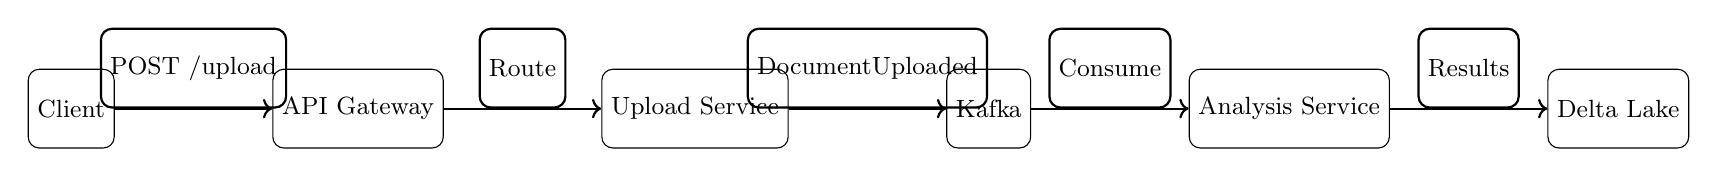
\begin{tikzpicture}[node distance=2cm, auto, every node/.style={rectangle, rounded corners, draw, minimum height=1cm, align=center, font=\small}]
    \node (client) {Client};
    \node[right=of client] (gateway) {API Gateway};
    \node[right=of gateway] (upload) {Upload Service};
    \node[right=of upload] (kafka) {Kafka};
    \node[right=of kafka] (analysis) {Analysis Service};
    \node[right=of analysis] (delta) {Delta Lake};
    \draw[->, thick] (client) -- node {POST /upload} (gateway);
    \draw[->, thick] (gateway) -- node {Route} (upload);
    \draw[->, thick] (upload) -- node {DocumentUploaded} (kafka);
    \draw[->, thick] (kafka) -- node {Consume} (analysis);
    \draw[->, thick] (analysis) -- node {Results} (delta);
\end{tikzpicture}
\end{processflow}

\section{Kafka Connect for Bulk Ingestion}
Kafka Connect integrates external systems with Kafka for bulk data ingestion.

\begin{glossaryterm}
\textbf{Kafka Connect}\newline
Kafka Connect is a framework for streaming data between Kafka and external systems (e.g., S3, databases).

\textbf{Key Characteristics}:
\begin{itemize}
    \item \textbf{Source/Sink}: Source connectors ingest data, sink connectors export data.
    \item \textbf{Scalability}: Distributed workers handle parallel tasks.
    \item \textbf{Fault Tolerance}: Retries and Dead Letter Queues (DLQs) handle failures.
    \item \textbf{Role in EDA}: Bridges external data sources to Kafka events.
\end{itemize}

\textbf{Inputs/Outputs}:
\begin{itemize}
    \item \textbf{Inputs}: External data (e.g., S3 files, database rows).
    \item \textbf{Outputs}: Kafka events or external writes (e.g., to Delta Lake).
\end{itemize}

\textbf{Process Flow}:
\begin{enumerate}
    \item Source connector polls external system (e.g., S3 bucket).
    \item Converts data to Kafka records (e.g., Avro format).
    \item Writes records to topic (e.g., bulk-uploads).
\end{enumerate}

\textbf{Benefits}:
\begin{itemize}
    \item \textbf{Scalability}: Handles 100K files/day with distributed workers.
    \item \textbf{Reusability}: Pre-built connectors reduce development time.
\end{itemize}

\textbf{Example}: S3 Source Connector ingests tenant PDFs from S3 to Kafka.

\textbf{Analogy}: Kafka Connect is a conveyor belt moving goods between warehouses.

\textbf{Capstone Connection}: Ingests bulk tenant PDFs for LLaMA 3 processing.
\end{glossaryterm}

\begin{minted}[frame=single,fontsize=\small,bgcolor=codebg]{json}
{
  "name": "s3-source",
  "config": {
    "connector.class": "io.confluent.connect.s3.S3SourceConnector",
    "tasks.max": "10",
    "s3.bucket.name": "documents-bucket",
    "topics": "bulk-uploads",
    "format.class": "io.confluent.connect.s3.format.avro.AvroFormat",
    "key.converter": "io.confluent.connect.avro.AvroConverter",
    "value.converter": "io.confluent.connect.avro.AvroConverter",
    "s3.region": "us-east-1",
    "errors.tolerance": "all",
    "errors.deadletterqueue.topic.name": "dlq-bulk-uploads"
  }
}
\end{minted}

\begin{technote}
\textbf{Technical Note: Kafka Connect Optimization}\newline
Tune \texttt{tasks.max} based on partition count (e.g., 10 tasks for 10 partitions). Use DLQs for failed records. Monitor connector lag with Prometheus.\footnote{DLQs prevent data loss during ingestion failures.}
\end{technote}

\section{Lab: Microservice with Kafka Connect}
This lab builds a microservice and configures Kafka Connect for bulk ingestion.

\textbf{Steps}:
\begin{enumerate}
    \item Develop Spring Boot upload service with REST API.
    \item Configure S3 Source Connector to ingest PDFs.
    \item Test end-to-end flow with Testcontainers.
\end{enumerate}

\section{Exercises}
\begin{enumerate}
    \item Design microservices for upload, analysis, and archival processes.
    \item Configure JDBC sink connector to write analysis results to PostgreSQL.
    \item Implement a choreography-based saga for upload-to-archival workflow.
\end{enumerate}

\end{document}